% !TEX encoding = UTF-8
% !TEX TS-program = pdflatex
% !TEX root = ../tesi.tex
% !TEX spellcheck = it-IT

%**************************************************************
\chapter{Progettazione e codifica}
\label{cap:progettazione-codifica}
%**************************************************************
\section{Progettazione del database}
\label{sec:progettazione}
Dall'analisi dei requisiti del database è stato possibile ricavare lo schema del database da implementare. Nel presente documento non è possibile riportare completamente tale schema a causa delle sue grandi dimensioni, ne verranno dunque descritti e riportati i dettagli salienti. \bigskip

Per ottenere lo schema finale è stato innanzitutto modellato uno schema concettuale di base, tale schema è stato successivamente ristrutturato in modo da:

\begin{itemize}
	\item Eliminare le \gls{ridondanza}\glsfirstoccur{} non necessarie;
	\item Eliminare le gerarchie: \gls{mysql}\glsfirstoccur{} non consente la rappresentazione diretta di una gerarchia, si deve quindi trasformare tale costrutto in modo che possa essere implementato;
	\item Partizionare le relazioni N-N: tali relazioni sono da evitare in quanto portano ad avere valori duplicati in entrambe le entità che vi partecipano. La presenza di valori duplicati implica una maggiore complessità nella risoluzione delle query e, quindi, un abbassamento generale delle performance. Per ovviare a questo problema sono state introdotte varie \textit{entità aggregate} per dividere una relazione N-N in due relazioni 1-N o 0-N.
\end{itemize}

\subsection{Dizionario delle entità} %**************************
La tabella seguente documenta il significato delle entità rappresentate nello schema finale del database, in modo da evitare quanto più possibile situazioni di ambiguità. \\

Ogni entità è dotata degli attributi: id, created\_at, updated\_at. Questi non sono stati riportati nel dizionario delle entità, in quanto sono stati messi in risalto solo gli attributi caratteristici di ogni entità.

\begin{longtabu} to \textwidth {l X[2] X}
	\toprule
	\textbf{Entità} & \textbf{Descrizione} & \textbf{Attributi}\\
	\midrule
	\endhead
	users                            & Utenti iscritti a solo scopo di gioco     & name,\par surname,\par email,\par password,\par remember\_token \\ \midrule
external\_auth                   & Token di autenticazione fornito da un servizio esterno                               & external\_uid                                                                             \\ \midrule
admins                           & Utenti con accesso al solo CMS                                                       & name,\par surname,\par email,\par password,\par remember\_token                                           \\ \midrule
invitations                      & Inviti mandati e ricevuti dagli utenti     &                                                                                           \\ \midrule
logs                             & Log generati dalle richieste HTTP effettuate dagli user nel gioco                    & method,\par url,\par user\_ip\_address,\par user\_agent,\par additional\_data                             \\ \midrule
regions                          & Aree geografiche previste dal gioco                                                  & name                                                                                      \\ \midrule
timezones                        & Fusi orari previsti dal gioco                                                        & code,\par name,\par offset                                                                        \\ \midrule
business\_roles                  & Ambiti lavorativi previsti dal gioco                                                 & name                                                                                      \\ \midrule
languages                        & Lingue supportate dal gioco                                                          & locale,\par code                                                                              \\ \midrule
translatable\_contents           & I contenuti traducibili del gioco, ovvero quei contenuti che possono essere tradotti & default\_text                                                                             \\ \midrule
translations                     & Tutte le traduzioni disponibili relativamente ai contenuti traducibili presenti nel gioco             & text                                                                                      \\ \midrule
teams                            & Squadre presenti nel gioco                                                           & name, cover\_image                                                                        \\ \midrule
missions                         & Mission previste dal gioco                                                           & cover\_image, is\_visible, start\_date, end\_date                                         \\ \midrule
text\_posts                      & I post di tipo testo                                                                 & is\_visible                                                                               \\ \midrule
captcha\_posts                   & I post di tipo captcha                                                               & is\_visible                                                                               \\ \midrule
team\_posts                      & I post di tipo team                                                                  & is\_visible,\par time\_limit                                                                  \\ \midrule
user\_questions                  & Domande rivolte ai singoli utenti                                                    &                                                                                           \\ \midrule
user\_correct\_answers           & Le risposte corrette previste per le domande rivolte ai singoli utenti                                & content                                                                                   \\ \midrule
user\_questions\_business\_roles & Associazione tra le domande rivolte ai singoli utenti e le aree lavorative alle quali sono indirizzate. In questo modo, ogni possibile user\_question può essere indirizzata a tutti quegli utenti aventi il medesimo business\_role       &                                                                                           \\ \midrule
made\_user\_questions            & Associazione tra gli utenti e le domande ad essi effettivamente rivolte              &                                                                                           \\ \midrule
user\_answers                    & Risposte fornite dagli utenti in merito alle domande ad essi effettivamente rivolte                      & content, is\_correct                                                                      \\ \midrule
team\_questions                  & Domande rivolte ai team                                                              &                                                                                           \\ \midrule
team\_correct\_answers           & Le risposte corrette previste per le domande rivolte ai team                                & content                                                                                   \\ \midrule
made\_team\_questions            & Associazione tra i team e le domande ad essi effettivamente rivolte                  &                                                                                           \\ \midrule
team\_answers                    & Risposte fornite dai team in merito alle domande ad essi effettivamente rivolte                      & content, is\_correct                                                                      \\ \midrule
scores                           & Punteggi ottenuti dai team nel completare le varie mission                           & points \\
	\bottomrule \\
	\caption{Dizionario delle entità} \\
\end{longtabu}

\subsection{Dizionario delle relazioni} %**************************
La tabella seguente documenta il significato delle relazioni rappresentate nello schema finale del database, in modo da evitare quanto più possibile situazioni di ambiguità. \\
La colonna "Entità" riporta le entità partecipanti alla relazione, accompagnate dalla loro cardinalità.

\begin{longtabu} to \textwidth {l X[2] X}
	\toprule
	\textbf{Relazione} & \textbf{Descrizione} & \textbf{Entità}\\
	\midrule
	\endhead
	have       & Associa un utente di gioco con il proprio token di autenticazione esterno            & users (0,1)\par external\_auth (1,1) \\ \midrule
do           & Associa un utente di gioco con gli inviti da esso spediti                            & users (0,N)\par invitations (1,1)   \\ \midrule
receive      & Associa un utente di gioco con gli inviti da esso ricevuti                           & users (0,N)\par invitations (1,1)   \\ \midrule
produce      & Associa un utente di gioco con i log prodotti dalle sue richieste HTTP               & users (0,N)\par logs (1,1)   \\ \midrule
belong      & Associa un utente di gioco con l'area geografica alla quale appartiene                & users (0,1)\par regions (0,N)   \\ \midrule
belong      & Associa un'area geografica con il fuso orario al quale appartiene                     & regions (1,1)\par timezones (0,N)   \\ \midrule
have      & Associa un utente di gioco con l'ambito lavorativo al quale appartiene                  & users (0,1)\par business\_roles (0,N)   \\ \midrule
speak      & Associa un utente di gioco alla sua lingua preferita                                   & users (1,1)\par languages (0,N)   \\ \midrule
address      & Associa ogni traduzione alla propria lingua                                          & translations (1,1)\par languages (0,N)   \\ \midrule
have         & Associa un contenuto traducibile con tutte le sue traduzioni disponibili             & translatable\_contents (0,N)\par translations (1,1)   \\ \midrule
have         & Associa un utente al team al quale appartiene                                        & users (0,1)\par teams (0,N)   \\ \midrule
name         & Associa una mission al contenuto traducibile che rappresenta il nome della mission stessa & missions (1,1)\par translatable\_contents (1,1)   \\ \midrule
have         & Associa un post di tipo testo con la mission alla quale appartiene                   & text\_posts (1,1)\par missions (0,N)   \\ \midrule
have         & Associa un post di tipo captcha con la mission alla quale appartiene                 & captcha\_posts (1,1)\par missions (0,N)   \\ \midrule
have         & Associa un post di tipo team con la mission alla quale appartiene                    & team\_posts (1,1)\par missions (0,N)   \\ \midrule
content      & Associa un post di tipo testo al contenuto traducibile che rappresenta il corpo del post stesso                  																																						& text\_posts (1,1)\par translatable\_contents (1,1)   \\ \midrule
abstract      & Associa un post di tipo captcha al contenuto traducibile che rappresenta il corpo del post stesso                  																																						& captcha\_posts (1,1)\par translatable\_contents (1,1)   \\ \midrule
abstract      & Associa un post di tipo team al contenuto traducibile che rappresenta il corpo del post stesso                  																																						& team\_posts (1,1)\par translatable\_contents (1,1)   \\ \midrule
choose        & Associa un post di tipo captcha al bacino delle domande che possono essere rivolte ai singoli utenti                																																						  & captcha\_posts (0,N)\par user\_questions (1,1)   \\ \midrule
choose        & Associa un post di tipo team al bacino delle domande che possono essere rivolte ai team                																																						     & team\_posts (0,N)\par team\_questions (1,1)   \\ \midrule
content       & Associa una domanda utente al contenuto traducibile che rappresenta il corpo della domanda stessa                  																																						& user\_questions (1,1)\par translatable\_contents (1,1)   \\ \midrule
content       & Associa una domanda di tipo team al contenuto traducibile che rappresenta il corpo della domanda stessa                  																																						& team\_questions (1,1)\par translatable\_contents (1,1)   \\ \midrule
have          & Associa una domanda utente alle risposte corrette previste per la domanda stessa	  & user\_questions (1,N)\par user\_correct\_answers (1,1)   \\ \midrule
aggregate     & Collega una associazione tra domanda utente e ambito lavorativo con la rispettiva domanda utente. Questa relazione nasce dalla scomposizione della relazione N-N che legava una domanda utente con gli ambiti lavorativi ai quali è rivolta	    & user\_questions\_business\_roles (1,1)\par user\_questions (0,N)\\ \midrule
aggregate     & Collega una associazione tra domanda utente e ambito lavorativo con il rispettivo ambito lavorativo. Questa relazione nasce dalla scomposizione della relazione N-N che legava una domanda utente con gli ambiti lavorativi ai quali è rivolta	    & user\_questions\_business\_roles (1,1)\par business\_roles (0,N)\\ \midrule
aggregate     & Collega una associazione tra domanda utente e l'utente al quale è stata rivolta con la rispettiva domanda utente. Questa relazione nasce dalla scomposizione della relazione N-N che legava una domanda utente con l'utente al quale è rivolta    & made\_user\_questions (1,1)\par user\_questions (0,N)\\ \midrule
aggregate     & Collega una associazione tra domanda utente e l'utente al quale è stata rivolta con l'utente stesso. Questa relazione nasce dalla scomposizione della relazione N-N che legava una domanda utente con l'utente al quale è rivolta    & made\_user\_questions (1,1)\par users (0,N)\\ \midrule
aggregate     & Collega una associazione tra domanda di tipo team e il team al quale è stata rivolta con la rispettiva domanda di tipo team. Questa relazione nasce dalla scomposizione della relazione N-N che legava una domanda di tipo team con il team al quale è rivolta    & made\_team\_questions (1,1)\par team\_questions (0,N)\\ \midrule
aggregate     & Collega una associazione tra domanda utente e l'utente al quale è stata rivolta con il team stesso. Questa relazione nasce dalla scomposizione della relazione N-N che legava una domanda di tipo team con il team al quale è rivolta    & made\_team\_questions (1,1)\par teams (0,N)\\ \midrule
refer     & Collega una associazione tra domanda utente e l'utente al quale è stata rivolta con le risposte fornite per tale domanda dall'utente coinvolto   & made\_user\_questions (0,N)\par user\_answers (1,1)\\ \midrule
refer     & Collega una associazione tra domanda di tipo team e il team al quale è stata rivolta con le risposte fornite per tale domanda dal team coinvolto   & made\_team\_questions (0,N)\par team\_answers (1,1)\\ \midrule
give     & Associa una risposta fornita per una domanda utente all'utente che l'ha effettivamente fornita   & user\_answers (1,1)\par users (0,N)\\ \midrule
give     & Associa una risposta fornita per una domanda di tipo team al team che l'ha effettivamente fornita   & team\_answers (1,1)\par teams (0,N)\\ \midrule
unveil     & Collega una associazione tra domanda di tipo team e il team al quale è stata rivolta con l'utente che ha svelato la domanda avviando il timer   & made\_team\_questions (0,1)\par users (0,N)\\ \midrule
have     & Associa un team ai punteggi ottenuti nella risoluzione delle varie mission   & teams (0,N)\par scores (1,1)\\ \midrule
have     & Associa un punteggio con la mission nella quale è stato ottenuto   & scores (1,1)\par missions (0,N)\\ 
	\bottomrule \\
	\caption{Dizionario delle relazioni} \\
\end{longtabu}


\subsection{Regole di vincolo} %**************************
Alcuni vincoli e proprietà non sono immediatamente deducibili dallo schema del database, è stato quindi deciso di mettere per iscritto tali proprietà in modo da aumentare la chiarezza della progettazione:
\begin{enumerate}
	\item Ogni utente può inviare al più un invito a qualsiasi altro utente;
	\item Un utente può scegliere un'unica lingua preferita;
	\item Un utente può afferire al più ad un ambito lavorativo;
	\item Un utente può appartenere al più ad un'area geografica;
	\item Uno punteggio deve appartenere ad un unico team e può riferirsi ad un'unica mission completata da tale team;
	\item Un post deve appartenere ad un'unica mission;
	\item Una domanda utente deve appartenere ad un unico post di tipo captcha;
	\item Una domanda di tipo team deve appartenere ad un unico post di tipo team;
	\item Una domanda di tipo team può essere svelata al più da un utente;
	\item Un'area geografica deve appartenere ad un unico fuso orario;
	\item Una risposta corretta deve riferirsi ad un'unica domanda;
	\item Una risposta deve riferirsi ad un'unica domanda;
	\item Un log deve riferirirsi ad un unico utente;
	\item Una traduzione deve riferirsi ad un unico contenuto traducibile e ad un'unica lingua.
\end{enumerate}

%**************************************************************
\section{Progettazione ed implementazione del CMS}
\subsection{Descrizione dell'architettura}
Il framework Laravel agevola l'adozione del pattern architetturale \textbf{model-view-controller (MVC)}, che impone la suddivisione della \textit{business logic} dalla \textit{presentation logic}. Nelle applicazioni Laravel, la business logic coincide spesso con modelli di dati persistenti in un database mentre la presentation logic si concretizza in una serie di pagine web. \\
Il pattern MVC prevede tre componenti principali: \textbf{model}, \textbf{view} e \textbf{controller}.

\begin{figure}
	\centering
  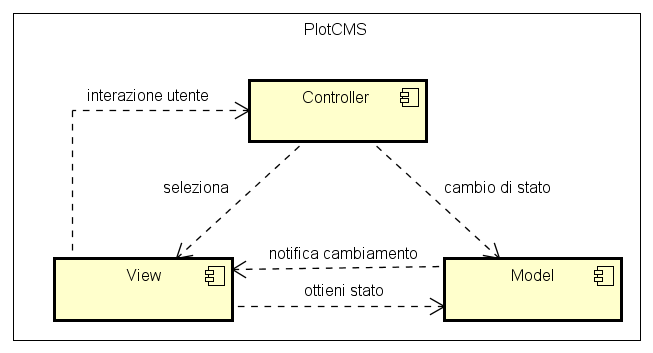
\includegraphics[scale=0.7]{immagini/components/mvc_diagram.png}
  \caption{Diagramma delle componenti del pattern MVC}
	\label{fig:mvc} 
\end{figure}

\subsubsection{Model} %****************************************************************
Il model rappresenta il dominio dell'applicazione e contiene l'astrazione di tutti i dati necessari al buon funzionamento della piattaforma. Nello specifico, esiste un'istanza di model per ogni entità prevista dal database collegato alla piattaforma, questo permette ed agevola l'interazione con il database attraverso l'\gls{orm}\glsfirstoccur{} Eloquent. \\
È compito del model notificare alla view eventuali cambiamenti avvenuti a livello del database, in modo da mostrare all'utente sempre e solo i dati aggiornati. \\
Le convenzioni del framework Laravel consigliano di posizionare le istanze del model nella directory \verb!app/Models!.

%**************************************************************************************

\subsubsection{View} %****************************************************************
La view è la rappresentazione visuale del model, cattura gli input dell'utente e ne delega l'elaborazione al controller. Nello specifico, l'interfaccia utente è composta da diverse pagine web che possono essere utilizzate dagli amministratori del \gls{cms}\glsfirstoccur{} per accedere alle varie funzionalità da esso offerte. \\
Le convenzioni del framework Laravel consigliano di posizionare le istanze della view nella directory \verb!resources/view!.

%**************************************************************************************

\subsubsection{Controller} %****************************************************************
Il controller coordina e crea un collegamento tra view e model, è responsabile quindi dell'elaborazione dell'input e dell'interazione con il model. \\
Le convenzioni del framework Laravel consigliano di posizionare le istanze del controller nella directory \verb!app/Http/Controllers!.

\begin{figure}
	\centering
  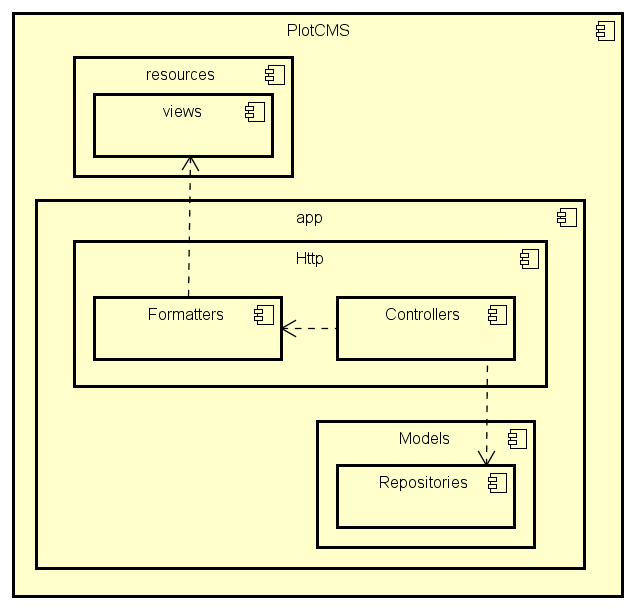
\includegraphics[scale=0.6]{immagini/components/important_components_diagram.png}
  \caption{Organizzazione delle principali componenti della piattaforma}
	\label{fig:components} 
\end{figure}

%**************************************************************
\section{Descrizione delle classi}
Di seguito sono descritte le classi e le interfacce più significative che compongono il \gls{cms}\glsfirstoccur{}, suddivise in base alla componente alla quale appartengono. \\
Le classi appartenenti alla stessa componente hanno spesso implementazione simile in quanto, di base, permettono il compimento delle azioni \gls{crud}\glsfirstoccur{} su risorse di tipo diverso. Per evitare di appesantire la documentazione, è stato scelto di fornire un esempio di classe laddove la descrizione di tutte le classi avrebbe reso il testo fortemente ridondante. \\
Le classi appartenenti al framework sono state evidenziate in arancio nei diagrammi che le prevedono, in modo da poterle individuare facilmente.

\subsection{app::Models} %*******************************************************************************************

Le classi appartenenti a questa componente forniscono un'astrazione delle entità presenti nel database collegato alla piattaforma e sono utilizzate per interagire con esse. \\
L'\gls{orm}\glsfirstoccur{} \textit{Eloquent} richiede che tutti i model espongano particolari metodi utili a descrivere le relazioni esistenti tra le entità rappresentate dai model stessi a livello di database.

\begin{figure}[H]
	\centering
  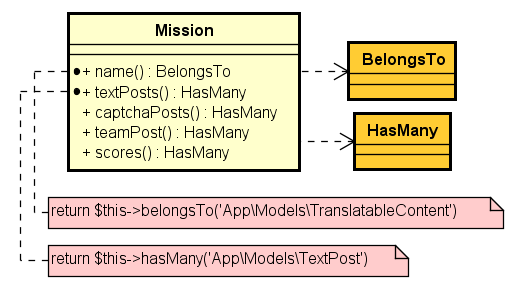
\includegraphics[scale=0.7]{immagini/components/mission.png}
  \caption{Diagramma della classe Mission}
	\label{fig:mission} 
\end{figure}

Ad esempio, la classe Mission prevede i seguenti metodi:

\begin{itemize}
	\item \verb!name()!: rappresenta la relazione con cardinalità 1-1 tra una mission ed il contenuto traducibile che corrisponde al nome della mission stessa;
	\item \verb!textPosts()!: rappresenta la relazione con cardinalità 0-N tra una mission ed i post di tipo testo collegati alla stessa;
	\item \verb!captchaPosts()!: rappresenta la relazione con cardinalità 1-N tra una mission ed i post di captcha testo collegati alla stessa;
	\item \verb!teamPosts()!: rappresenta la relazione con cardinalità 1-N tra una mission ed i post di tipo team collegati alla stessa;
	\item \verb!scores()!: rappresenta la relazione con cardinalità 1-N tra una mission ed i punteggi totalizzati dai team relativamente alla mission stessa.
\end{itemize}

\begin{figure}[H]
	\centering
  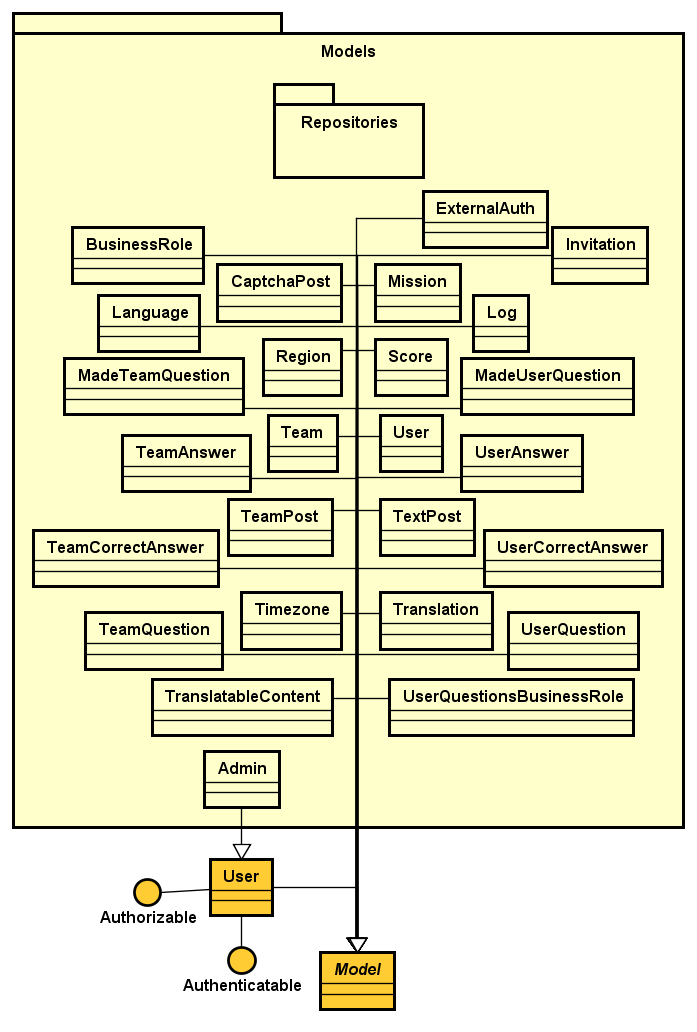
\includegraphics[scale=0.55]{immagini/components/models_diagram.png}
  \caption{Diagramma delle classi della componente Models}
	\label{fig:models} 
\end{figure}

Maggiori dettagli sui metodi esposti dall'\gls{orm}\glsfirstoccur{} Eloquent per rappresentare le relazioni tra model possono essere recuperati nella documentazione online ufficiale del framework Laravel (\cite{site:laravel-doc}).


\subsubsection{app::Models::Repositories} %*******************************************************************************************

\begin{figure}[H]
	\centering
  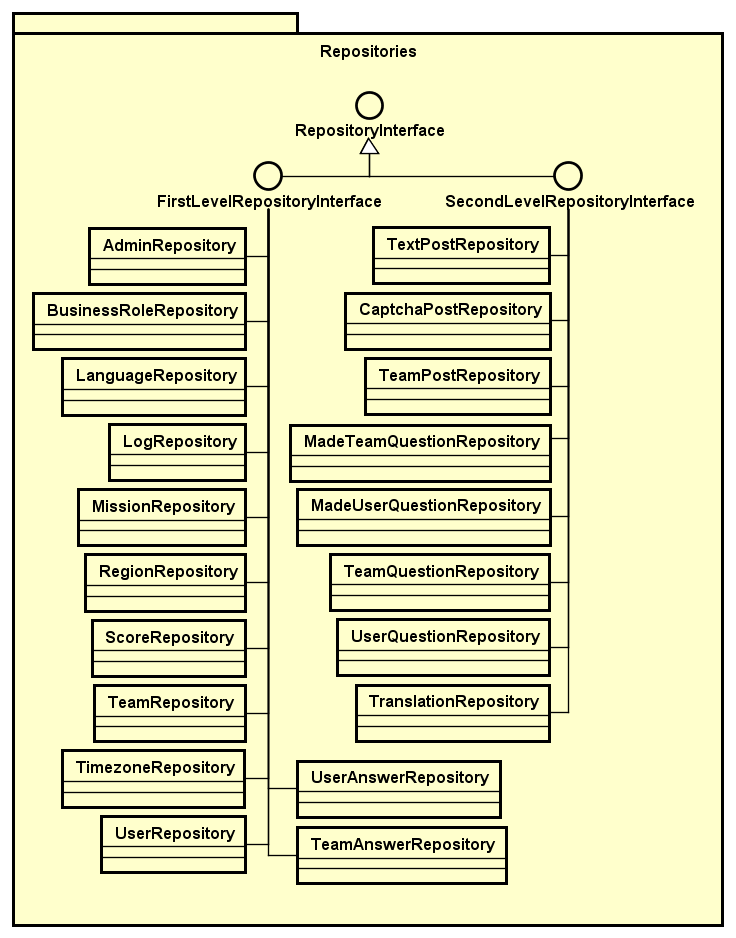
\includegraphics[scale=0.6]{immagini/components/repositories_diagram.png}
  \caption{Diagramma delle classi della componente Repositories}
	\label{fig:repositories} 
\end{figure}

Le classi e le interfacce appartenenti a questa componente sono utilizzate per implementare il design pattern \textbf{Repository}, utile per disaccoppiare la \textit{business logic} dal sistema di persistenza dati effettivamente utilizzato. In questo modo le istanze del controller possono effettuare query in modo dichiarativo sulle istanze del model, lasciando che siano i repository ad occuparsi dei dettagli implementativi delle query stesse. \\
Concettualmente, un repository incapsula l'insieme delle operazioni disponibili sulle entità di un database, così da fornire un modo più \textit{object-oriented} per accedervi.\\ \\

Le istanze di repository possono essere fondamentalmente di due tipi, in base al model che devono trattare:
\begin{itemize}
	\item \textbf{First level}: se l'istanza del repository è collegata ad un model la cui esistenza è autoesplicativa, ovvero non necessita di un secondo model; 
	\item \textbf{Second level}: se l'istanza del repository è collegata ad un model che ha senso di esistere solo come figlio di un secondo model. Un esempio di questa tipologia è TextPostRepository, collegato al model TextPost le cui istanze sono significative solo come figlie di un'istanza di Mission.
\end{itemize}

\begin{figure}[H]
	\centering
  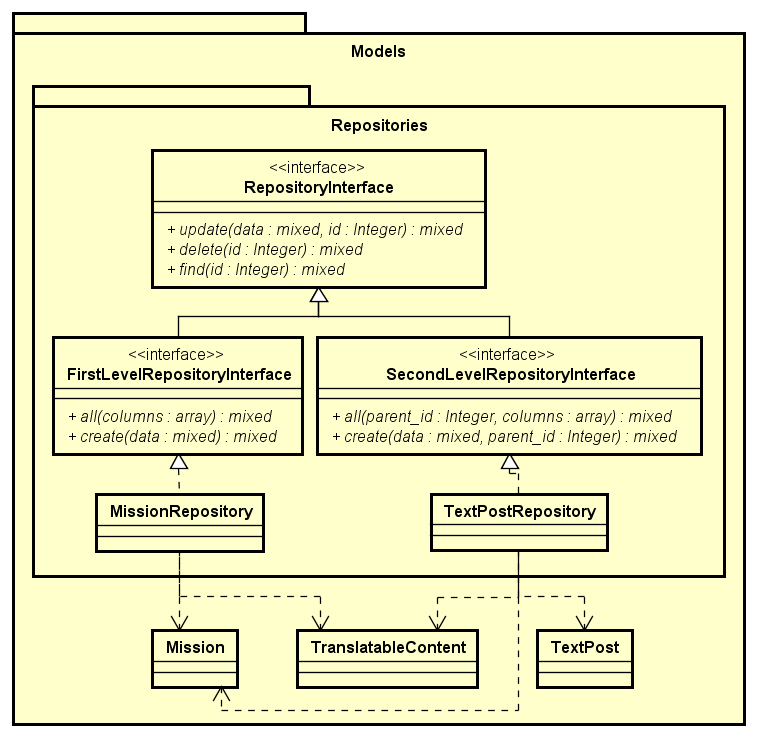
\includegraphics[scale=0.7]{immagini/components/repository_example.png}
  \caption{Diagramma delle classi MissionRepository e TextPostRepository}
	\label{fig:repository-example} 
\end{figure}

\newpage
Per modellare la situazione sopra descritta sono state usate delle interfacce:
\begin{itemize}
	\item \textbf{Repositories::RepositoryInterface}: espone metodi per effettuare l'aggiornamento, la rimozione o il recupero di particolari risorse. Tali metodi sono indipendenti dal tipo di repository;
	\item \textbf{Repositories::FirstLevelRepositoryInterface}: espone metodi per effettuare il recupero e la creazione di risorse che non prevedono una risorsa padre. Estende \verb!RepositoryInterface!;
	\item \textbf{Repositories::SecondLevelRepositoryInterface}: espone metodi per effettuare il recupero e la creazione di risorse che necessitano di una risorsa padre. Estende \verb!RepositoryInterface!.
\end{itemize}

Un esempio di repository \textit{first level} è MissionRepository, mentre un esempio di repository \textit{second level} è TextPostRepository. Il secondo differisce dal primo a causa del parametro \verb!parent_id!, necessario per individuare il padre della risorsa da creare e/o recuperare.

\subsection{resources::views} %******************************************************************************************

\begin{figure}[H]
	\centering
  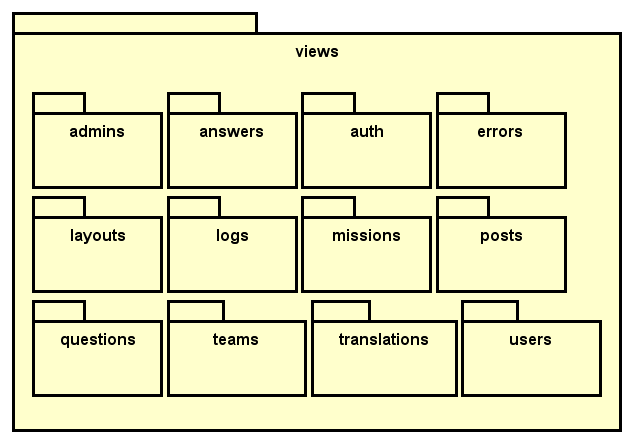
\includegraphics[scale=0.7]{immagini/components/views_diagram.png}
  \caption{Diagramma delle classi della componente views}
	\label{fig:views} 
\end{figure}

I file appartenenti a questa componente costituiscono l'interfaccia utente del \gls{cms}\glsfirstoccur{}, accessibile attraverso un browser web. L'interfaccia utente è stata ottenuta utilizzando i widget messi a disposizione dal template Bootstrap "Gentelella", liberamente disponibile online all'indirizzo \url{https://github.com/puikinsh/gentelella}. La scelta per la realizzazione dell'interfaccia utente è ricaduta sull'utilizzo di un template in modo da poter contenere i tempi di progettazione, senza dover per questo rinunciare alla qualità visiva e funzionale.\\

Per aumentare la modularizzazione delle view e la loro manutenibilità è stato utilizzato \textbf{Blade}: il \textit{template system} offerto dal framework Laravel. Grazie a Blade è possibile: 

\begin{itemize}
	\item Definire dei \textit{template} che fungano da base per la costruzione di diverse view;
	\item Utilizzare delle scorciatoie che agevolano azioni comunemente effettuate dalle view sui dati che devono mostrare, come stampare il valore di una variabile o scorrere una struttura dati.
\end{itemize}

L'utilizzo dei template ha reso possibile introdurre il concetto di ereditarietà, seppur abbastanza superficiale, nell'ambito HTML che ne è storicamente sprovvisto. \\
I file contenenti le view sono poi stati suddivisi sulla base del model al quale sono collegati. Ad esempio, nella sotto-componente \textbf{views::missions} sono contenuti i file:

\begin{itemize}
	\item \textbf{all.blade}: struttura della view che mostra la lista di tutte le mission previste dal gioco;
	\item \textbf{create.blade}: struttura della view che presenta il form utile per creare una nuova mission;
	\item \textbf{edit.blade}: struttura della view che mostra il form utile a modificare i dettagli di una mission esistente;
	\item \textbf{show.blade}: struttura della view che mostra i dettagli di una mission esistente.
\end{itemize}

La sotto-componente più importante è \textbf{views::layouts} che contiene il file \textbf{app.blade}. Questo file definisce la base di ogni pagina web, una struttura a tre pannelli che prevede: 

\begin{itemize}
	\item Un menù di navigazione che riporta le sezioni più importanti del sito;
	\item Il nome dell'utente autenticato, associato alla possibilità di effettuare il logout;
	\item Il contenuto della pagina, provvisto dei dati richiesti dall'utente.
\end{itemize}

Tutte le view estendono \textbf{app.blade} in modo da mantenere un \textit{look-and-feel} consistente per l'intero sito.

\subsection{app::Http::Controllers} %*******************************************************************************************

Le classi e le interfacce appartenenti a questa componente sono deputate alla gestione delle richieste \gls{http}\glsfirstoccur{} in entrata: ogni richiesta viene inoltrata allo specifico controller in grado di soddisfarla. 
\\ \\
Nel framework Laravel, una \textit{route} rappresenta l'associazione tra una richiesta \gls{http}\glsfirstoccur{} e il controller utile alla sua risoluzione, tutte le route previste sono salvate nel file \verb!app/Http/routes.php!. 
Un esempio di route è il seguente:

\begin{lstlisting}[frame=none]
Route::get('missions.textposts','WebTextPostController@index')
\end{lstlisting}

Questa route indica che la piattaforma può gestire una richiesta \gls{http}\glsfirstoccur{} inoltrata all'\gls{url}\glsfirstoccur{} \verb!missions/mission_id/textposts/textpost_id! con metodo GET. La gestione è presa in carico dal metodo \verb!index! del controller \verb!WebTextPostController!. I segnaposto \verb!mission_id! e \verb!textpost_id! indicano che l'\gls{url}\glsfirstoccur{} prevede due parametri interi, positivi e non opzionali. Tali parametri rappresentano rispettivamente l'id del post di tipo testo che si vuole recuperare e l'id della mission alla quale il post è collegato. \\
Il passaggio dei parametri, contenuti nell'\gls{url}\glsfirstoccur{}, al metodo del controller viene completamente gestito dal framework Laravel: il primo parametro dell'\gls{url}\glsfirstoccur{} viene passato al primo parametro del metodo, il secondo parametro dell'\gls{url}\glsfirstoccur{} viene passato al secondo parametro del metodo e così via. 
Questa peculiarità implica che la struttura di ogni controller sia influenzata dal tipo di route che deve gestire, il tipo della particolare route dipende dal numero di parametri in essa presenti.\\ 
Sono stati quindi parametrizzati diversi tipi di controller:

\begin{itemize}
	\item \textbf{First level}: se il controller deve gestire una route con al più un parametro;
	\item \textbf{Second level}: se il controller deve gestire una route con al più due parametri;
	\item \textbf{Third level}: se il controller deve gestire una route con al più tre parametri;
	\item \textbf{Fourth level}: se il controller deve gestire una route con al più quattro parametri;
	\item \textbf{Fifth level}: se il controller deve gestire una route con al più cinque parametri.
\end{itemize}

Dall'analisi dei requisiti è emerso, inoltre, che la piattaforma deve essere accessibile sia attraverso un browser web sia attraverso le API REST esposte dalla stessa, sono stati quindi previsti due gruppi di route:

\begin{itemize}
	\item \textbf{Route web}: utilizzate per accedere all'interfaccia grafica del \gls{cms}\glsfirstoccur{} da browser web; 
	\item \textbf{Route API}: utilizzate per accedere alle API REST offerte dalla piattaforma. L'\gls{url}\glsfirstoccur{} per usufruire di una certa funzionalità attraverso una route API equivale all'\gls{url}\glsfirstoccur{} per accedere alla stessa funzionalità attraverso una route web, con l'aggiunta del prefisso \verb!api/v1!. Ad esempio, per accedere ad un'interfaccia grafica contenente la lista di tutte le mission è possibile utilizzare l'\gls{url}\glsfirstoccur{} \verb!/missions!, mentre per ottenere un pacchetto JSON contenente lo stesso risultato è possibile utilizzare l'\gls{url}\glsfirstoccur{} \verb!/api/v1/missions!.
\end{itemize}

La differenza tra i controller adibiti alla gestione delle route web e i controller adibiti alla gestione delle route API consiste nella sola formattazione del risultato restituito, questo ha portato all'utilizzo del design pattern \textbf{Template Method}. Il pattern Template Method permette di definire la struttura di un algoritmo lasciando alle sottoclassi il compito di implementarne alcuni passi, in questo modo è possibile ridefinire e personalizzare parte del comportamento nelle sottoclassi evitando codice duplicato. \\ 
La struttura dell'algoritmo è solitamente definita in un metodo chiamato \textit{template method}, tale metodo utilizza delle \textit{operazioni primitive} astratte che devono essere concretizzate dalle sottoclassi per specializzarne il comportamento. 

\begin{figure}[H]
	\centering
  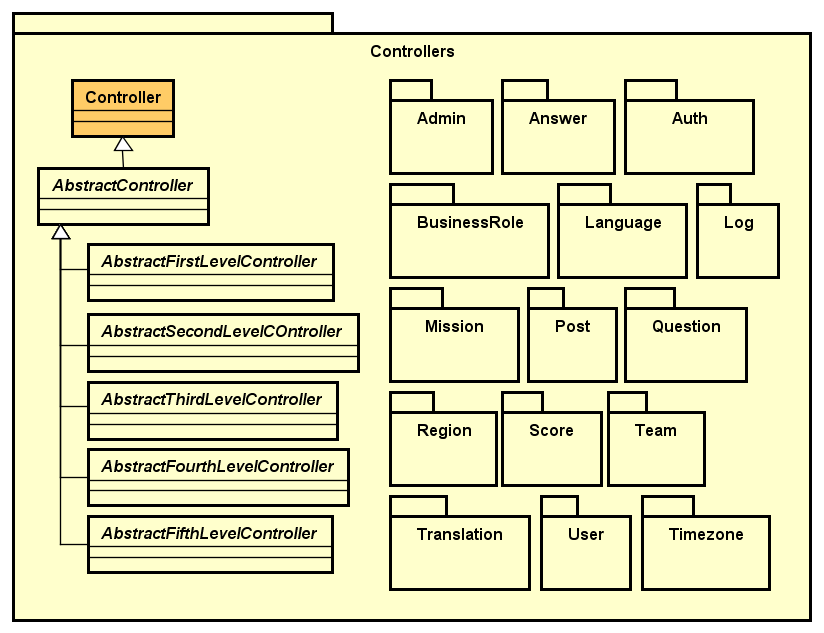
\includegraphics[scale=0.95, width=\textwidth]{immagini/components/controllers_diagram.png}
  \caption{Diagramma delle classi della componente Controllers}
	\label{fig:controllers} 
\end{figure}

Per modellare la situazione sopra descritta sono state utilizzate delle classi astratte:

\begin{itemize}
	\item \textbf{Controllers::AbstractController}: definisce l'attributo \verb!repository! che ospiterà il riferimento al principale repository utilizzato dalla classe che concretizza AbstractController. Per mantenere una struttura consistente, infatti, ogni controller non può accedere direttamente al model ma deve servirsi dell'apposito repository. Questa classe espone inoltre il metodo astratto \verb!format!, ovvero l'\textit{operazione primitiva} utilizzata dai metodi delle sottoclassi per restituire un risultato all'utente. Questo metodo deve essere implementato dalle sottoclassi in modo da restituire i dati nel formato corretto rispetto alla modalità d'accesso dell'utente alla piattaforma; 
	\item \textbf{Controllers::AbstractFirstLevelController}: definisce l'interfaccia dei controller di tipo \textit{first level};
	\item \textbf{Controllers::AbstractSecondLevelController}: definisce l'interfaccia dei controller di tipo \textit{second level};
	\item \textbf{Controllers::AbstractThirdLevelController}: definisce l'interfaccia dei controller di tipo \textit{third level};
	\item \textbf{Controllers::AbstractFourthLevelController}: definisce l'interfaccia dei controller di tipo \textit{fourth level};
	\item \textbf{Controllers::AbstractFifthLevelController}: definisce l'interfaccia dei controller di tipo \textit{fifth level}.
\end{itemize}

L'interfaccia dei controller è composta da una serie di metodi utili per: creare una nuova risorsa, recuperare una determinata risorsa, aggiornare una determinata risorsa, eliminare una determinata risorsa. \bigskip

Le classi appartenenti a questa componente adoperano il design pattern \textbf{Dependency Injection} per separare il loro comportamento dalla risoluzione delle dipendenze che espongono. In particolare questo pattern è utilizzato per \textit{iniettare}, utilizzando il costruttore della classe, le dipendenze relative ai repository usati da ogni controller.

\begin{figure}[H]
	\centering
  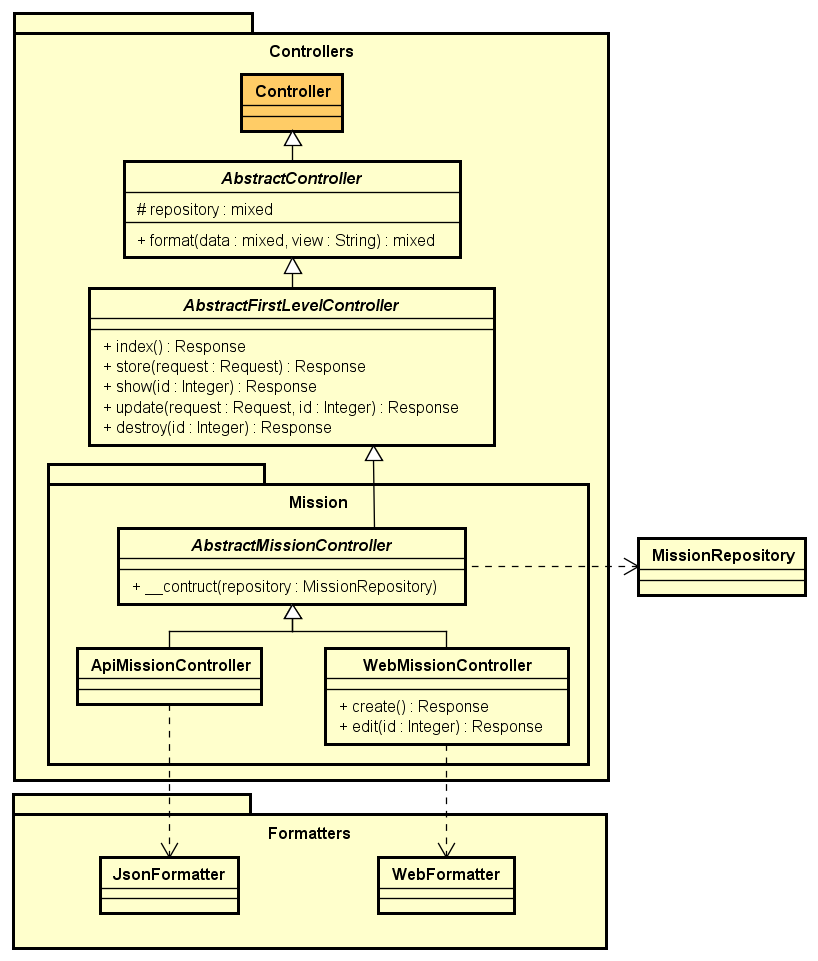
\includegraphics[scale=0.5, width=\textwidth]{immagini/components/controllers_example.png}
  \caption{Diagramma delle classi ApiMissionController e WebMissionController}
	\label{fig:controller-example} 
\end{figure}
 
Due esempi di controller di tipo \textit{first level} sono i controller adibiti alla gestione delle mission: ApiMissionController e WebMissionController. Questi controller derivano da \textbf{AbstractMissionController} che si occcupa di implementare i metodi ereditati da AbstractFirstLevelController. Le classi concrete \textbf{ApiMissionController} e \textbf{WebMissionController} hanno invece due compiti: 

\begin{itemize}
	\item Esporre eventuali metodi specifici e relativi ad una sola modalità di accesso, ad esempio i controller che gestiscono l'accesso tramite web (come WebMissionController) espongono metodi per mostrare i form utili alla creazione e aggiornamento delle risorse, questo non è necessario per i controller che gestiscono l'accesso tramite API (come ApiMissionController);
	\item Implementare il metodo astratto \verb!format!, utilizzando il costrutto appropriato della componente \hyperlink{formatters}{Formatters}.
\end{itemize} 

\hypertarget{formatters}{} %*******************************************************************************************
\subsection{app::Http::Formatters} 
\begin{figure}[H]
	\centering
  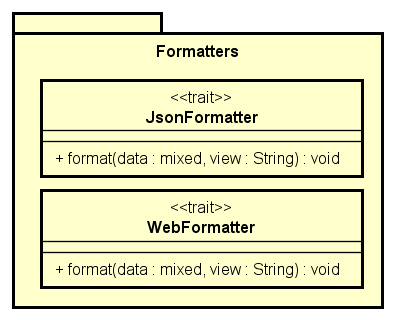
\includegraphics[scale=0.8]{immagini/components/formatters_diagram.png}
  \caption{Diagramma delle classi della componente Formatters}
	\label{fig:formatters} 
\end{figure}

La differenza fondamentale tra l'accesso tramite browser web e l'accesso tramite API REST riguarda la formattazione dei dati ottenuti come risultato della richiesta: 
\begin{itemize}
	\item Se l'accesso avviene tramite browser web, l'utente si aspetta di poter interagire con un'interfaccia grafica;
	\item Se l'accesso avviene tramite API REST, l'utente si aspetta di poter interagire con un formato di dati strutturato. In questo caso è stato scelto di fornire all'utente un pacchetto di dati in formato \gls{json}\glsfirstoccur{} in quando tale formato è oggi largamente utilizzato nello scambio di dati sul web, inoltre il framework Laravel ne rende molto agevole la manipolazione.
\end{itemize} 

Questa componente contiene due \gls{trait}\glsfirstoccur{} che si occupano proprio di formattare il risultato della richiesta in modo adeguato:
\begin{itemize}
	\item \textbf{Formatters::JsonFormatter}: restituisce i dati in formato \gls{json}\glsfirstoccur{};
	\item \textbf{Formatters::WebFormatter}: restituisce i dati attraverso una web view.
\end{itemize}

Entrambi i \gls{trait}\glsfirstoccur{} espongono un unico metodo: \verb!format!. Essi vanno intesi come dei pacchetti di codice pre-confezionato che agevolano lo sviluppatore nell'implementazione del metodo \verb!format! richiesto per la realizzazione di un controller concreto. In questo modo la scrittura di codice duplicato viene ridotta al minimo: lo sviluppatore deve solamente scegliere quale formatter utilizzare e non deve preoccuparsi di scrivere la procedura per la formattazione, in quanto questa è già incapsulata nel formatter scelto.




